	\section{Модель элементов картины мира}
	\subsection{Знаковая картина мира}
	
	\begin{frame}
		\frametitle{Картина мира субъекта деятельности}
		\scriptsize
		\onslide<1->{
			Картина мира субъекта деятельности - это представления субъекта о внешней среде, о своих собственных характеристиках, целях, мотивах, о других субъектах и операции (произвольные и непроизвольные), осуществляемые на основе этих представлений.
		}
		\onslide<2->{
			\par\smallskip
			Элементом картины мира является знак:
			\begin{itemize}
				\item в смысле культурно-исторического подхода Выготского-Лурии,
				\item выполняющий функции в соответствии с теорией деятельности Леонтьева.
			\end{itemize}
		}
		\onslide<3->{
			\begin{columns}
				\begin{column}{0.4\textwidth}
					\centering
					\includegraphics[width=0.6\textwidth]{signs/ru/sign_color_book_ru}
				\end{column}
		}
		\onslide<4->{
				\begin{column}{0.6\textwidth}
					\begin{columns}
						\begin{column}{0.5\textwidth}
							\centering
							\includegraphics[width=\textwidth]{misc/phisio/ivan_cyrc}
						\end{column}
						\begin{column}{0.5\textwidth}
							\centering
							\includegraphics[width=\textwidth]{misc/phisio/workspace}
						\end{column}
					\end{columns}
					
				\end{column}
			\end{columns}
			В пользу существования такой структуры свидетельствуют:
			\begin{itemize}
				\item нейрофизиологические данные (Эдельман, Иваницкий, Маунткастл и др.),
				\item другие психологические теории (например, трехкомпонентная модель Станович).
			\end{itemize}
			\vspace{-5pt}
			\nocite{*}
			\printbibliography[keyword={sign}, resetnumbers=true]
		}
	\end{frame}
	
	\begin{frame}
		\frametitle{Три образующих элемента картины мира}
		\footnotesize
		\begin{figure}
			\includegraphics[width=0.3\textwidth]{signs/ru/sign_colored}
		\end{figure}
		
		Представляемая сущность описывается тремя причинно-следственными (каузальными) структурами:
		\begin{itemize}
			\item {\color{red}структура образа} - представление взаимосвязи внешних сигналов и внутренних характеристик субъекта (агента) - сенсо-моторное представление,
			\item {\color{blue}структура значения} - обобщенное знание о соотношениях во внешнем мире, согласованное в некоторой группе субъектов (агентов),
			\item {\color{green!60!black}структура личностного смысла} - ситуационная потребностно-мотивационная интерпретация знаний о соотношениях во внешней среде (значение для себя).
		\end{itemize}
	\nocite{*}
	\printbibliography[keyword={qualia}, resetnumbers=true]
	\end{frame}

	\begin{frame}
		\frametitle{Актуализация и формирование знака}
		\begin{figure}
			\includegraphics[width=0.4\textwidth]{signs/en/sign_naming_colored_en}
		\end{figure}
		\small
		\textbf{Процесс обучения} "--- образование новых знаков как неподвижная точка операторов замыкания $\Psi_p^m\Psi_m^a\Psi_a^p$.
		\par\smallskip
		Реализация когнитивных функций "--- \textbf{актуализация} (активация) имеющихся знаков и формирование новых <<ситуационных>> знаков "--- <<протознаков>> без конвенционального имени.
	\end{frame}

	\begin{frame}
		\frametitle{Уровни представления}
		\begin{figure}
			\includegraphics[width=0.7\textwidth]{signs/ru/sign_levels}
		\end{figure}
	\end{frame}

	\subsection{Нейронный субстрат}

	\begin{frame}
		\frametitle{Нейронный субстрат}
		
		\begin{columns}
			\begin{column}{0.35\textwidth}
				\includegraphics[width=0.8\textwidth]{misc/phisio/mozg_2}
				\par\bigskip
				\hspace{-7mm}\includegraphics[width=\textwidth]{misc/phisio/mozg}
			\end{column}
			\begin{column}{0.65\textwidth}
				\includegraphics[width=\textwidth]{misc/phisio/cortex_layers}
			\end{column}
		\end{columns}
		\nocite{*}
		\printbibliography[keyword={column}, resetnumbers=true]
	\end{frame}

	
	\begin{frame}
		\frametitle{Гетерархическая модель}
		\scriptsize
		Разработана расширенная реализация иерархической временной памяти (hierarchical temporal memory - HTM) - \textbf{гетерархическая каузальная сеть (heterarchical causal network - HCN)}.
		
		\begin{center}
			\includegraphics[width=0.4\textwidth]{misc/mpf/hawkins_htm}
		\end{center}
		\nocite{*}
		\printbibliography[keyword={starthtm}, resetnumbers=true]
	\end{frame}

	\begin{frame}
		\frametitle{Гетерархическая модель}

		\begin{center}
			\includegraphics[width=0.3\textwidth]{misc/mpf/hawkins_htm_ex_a}
			\includegraphics[width=0.3\textwidth]{misc/mpf/hawkins_htm_ex_b}
		\end{center}
		\nocite{*}
		\printbibliography[keyword={hetermem}, resetnumbers=true]
	\end{frame}
		
	\begin{frame}
		\frametitle{Нейронная организация}
		
		\begin{columns}
			\begin{column}{0.65\textwidth}
				\includegraphics[width=0.9\textwidth]{misc/mpf/regions_connect}
			\end{column}
			\begin{column}{0.35\textwidth}
				\includegraphics[width=\textwidth]{misc/phisio/column}
			\end{column}
		\end{columns}
		\nocite{*}
		\printbibliography[keyword={simplehtm}, resetnumbers=true]
	\end{frame}
	
	\begin{frame}
		\frametitle{Модель процесса обучения}
		
		К основным принципам работы механизма обучения относятся: 
		
		\begin{itemize}
			\item использование иерархии вычислительных узлов с восходящими и нисходящими связями, 
			\item использование Хэббовских правил обучения, 
			\item разделение пространственного и временного группировщиков, 
			\item подавление второстепенной активации для формирования разреженного представления.
		\end{itemize}
		
		В результате работы механизма обучения по прецедентам (без учителя) формируются так называемые \textbf{каузальные матрицы}.
		\vfill
		\nocite{*}
		\printbibliography[keyword={htmlearn}, resetnumbers=true]
	\end{frame}	
	
	\subsection{Образная компонента знака}
	\begin{frame}
		\frametitle{Каузальная матрица}                             
		\centering
		\includegraphics[width=0.7\textwidth]{causnet/caus_matr}
		\vspace{10pt}
		\nocite{*}
		\printbibliography[keyword={per}, resetnumbers=true]
	\end{frame}

	\begin{frame}
		\frametitle{Алгоритм $\mathfrak A_{th}$ активации образа знака}
		
		\begin{tikzpicture}[overlay,remember picture]
		
		\tikzstyle{z_matrix} = [draw, rectangle, minimum width = 60, minimum height = 60,fill=white];
		
		\onslide<1->{
			\node (meas_fun) at (0.7,0.5) {$\hat f_1,\hat f_2\dots,\hat f_k$};	
		}
		\onslide<2->{
			\node (control_vect) at ($(meas_fun)+(-0.5,1.2)$) {$\hat x^{j+1}$};
			\path[->,thick,red] (control_vect.east)  edge[out = -45, in = 45, right] (meas_fun.north); 
		}
		\onslide<3->{
			\node[z_matrix] (z_1) at ($(meas_fun)+(2.6,-0.5)$) {};
			\node[z_matrix] at ($(z_1)+(0.2,-0.1)$) {};
			\node[z_matrix] at ($(z_1)+(0.4,-0.2)$) {};
			
			\node[z_matrix] at ($(z_1)+(0.9,-0.5)$) {};
			\node[z_matrix] at ($(z_1)+(1.1,-0.6)$) {};
			\node[z_matrix] at ($(z_1)+(1.3,-0.7)$) {};
			
			\path[->,thick,blue] ([xshift=20]meas_fun.south)  edge[out = -90, in = -155, right] ($(z_1)+(-1,-1.2)$);
			\path[->,thick,blue] ([xshift=-25]meas_fun.south)  edge[out = -90, in = -155, right] ($(z_1)+(-0.1,-1.7)$);
			
			\node at ($(z_1)+(-1,1.4)$) {$Z^*$};
			
			\node at ($(z_1)+(0.8,1.4)$) {$Z_1$};
			\node at ($(z_1)+(1.4,1.2)$) {$\ddots$};
			\node at ($(z_1)+(2,0.9)$) {$Z_k$};
		}
		
		\onslide<4->{
			\draw[ultra thick, green!60!black] ($(z_1)+(-0.4,-1.1)$) -- ($(z_1)+(-0.4,0.6)$);
			\draw[ultra thick, green!60!black] ($(z_1)+(0.5,-1.6)$) -- node[right,black] {$z_1^r$} ($(z_1)+(0.5,0.1)$);
			
			\draw[->, thick, green!60!black] ($(z_1)+(-0.1,-3)$) -- node[right,black] {$\bar x(0)$} ($(z_1)+(-0.1,-2)$);
		}
		
		\onslide<5->{
			\node[z_matrix] (z_2) at ($(z_1)+(5,0)$) {};
			\node[z_matrix] at ($(z_2)+(0.2,-0.1)$) {};
			
			\node[z_matrix] at ($(z_2)+(0.9,-0.5)$) {};
			\node[z_matrix] at ($(z_2)+(1.3,-0.7)$) {};
			
			\node at ($(z_2)+(-1,1.4)$) {$Z^*$};
			\node at ($(z_2)+(0.8,1.4)$) {$Z_1$};
			\node at ($(z_2)+(1.4,1.2)$) {$\ddots$};
			\node at ($(z_2)+(2,0.9)$) {$Z_k$};
			
			\draw[->, ultra thick] ($(z_1)+(2.6,-0.6)$) -- node [above] {\scriptsize$\frac{\|\bar z_1^r-\bar x(0)\|}{\|\bar z_1^r\|+\|\bar x(0)\|}$} ($(z_1)+(3.7,-0.6)$);
			
			\draw[ultra thick, dotted, green!60!black] ($(z_2)+(-0.6,-1)$) -- ($(z_2)+(-0.6,0.7)$);
			\draw[ultra thick, dotted, green!60!black] ($(z_2)+(0.5,-1.6)$) -- ($(z_2)+(0.5,0.1)$);
		}
		
		\onslide<6->{
			\draw[->, thick, red] ($(z_2)+(0.3,1.4)$) -- node[right,black] {$\bar x^*(0)$} ($(z_2)+(0.3,3)$);
		}
		
		\onslide<7>{
			\draw[<-, thick, red] ($(z_2)+(-0.1,-3)$) -- node[right,black] {$\hat x^j(0)$} ($(z_2)+(-0.1,-2)$);
		}
		
		\onslide<7->{				
			\draw[ultra thick, green!60!black] ($(z_2)+(-0.4,-1)$) -- ($(z_2)+(-0.4,0.7)$);
			\draw[ultra thick, green!60!black] ($(z_2)+(0.7,-1.6)$) -- node[right,black] {$z_2^r$} ($(z_2)+(0.7,0.1)$);	
		}
		\onslide<8->{
			\draw[->, thick, green!60!black] ($(z_2)+(-0.1,-3)$) -- node[right,black] {$\bar x(1)$} ($(z_2)+(-0.1,-2)$);
		}
		
		\onslide<9->{
			\draw[->, ultra thick] ($(z_2)+(2.6,-0.6)$) -- node [above] {\scriptsize$\frac{\|\bar z_1^r-\bar x(1)\|}{\|\bar z_1^r\|+\|\bar x(1)\|}$} ($(z_2)+(3.7,-0.6)$);
		}
		\end{tikzpicture}
		
	\end{frame}	

	\subsection{Каузальная сеть}
	\begin{frame}
		\frametitle{Каузальная сеть на образах}
		\footnotesize
		\textbf{Каузальная сеть} на множестве образов знаков $W_p=\langle V_p, E_p \rangle$ - помеченный ориентированный граф, в котором
		\begin{itemize}
			\item каждому узлу $v\in V_p$ ставится в соответствие кортеж казуальных матриц $Z^p(s)$ образа некоторого знака $s$ ($v\rightarrow Z^p(s)$);
			\item ребро $e=(v_1, v_2)$ принадлежит множеству ребер графа $E$, если $v_1\rightarrow Z^p(s_1), v_2\rightarrow Z^p(s_2)$ и $s_1\in S_p(s_2)$;
			\item каждому ребру графа $e=(v_1, v_2), v_1\rightarrow Z^p(s_1), v_2\rightarrow Z^p(s_2)$ ставится в соответствие метка $\epsilon=(\epsilon_1,\epsilon_2,\epsilon_3)$ - кортеж трех натуральных чисел:
			\begin{itemize}
				\item $\epsilon_1$ - индекс исходной матрицы в кортеже $Z^p(s_1)$, может принимать специальное значение 0, если исходными могут служить любые матрицы из кортежа;
				\item $\epsilon_2$ - индекс целевой матрицы в кортеже $Z^p(s_2)$, строка которой ставится в соответствие признаку $s_1$;
				\item $\epsilon_2$ - индекс столбца в целевой матрице, в которой в соответствующей признаку $s_1$ строке стоит 1, может принимать положительные значения (\textit{столбцы условий}) и отрицательные (\textit{столбцы эффектов}).
			\end{itemize}		
		\end{itemize}
	\end{frame}

	\begin{frame}
		\frametitle{Каузальная сеть на образах: пример}
		
		\centering
		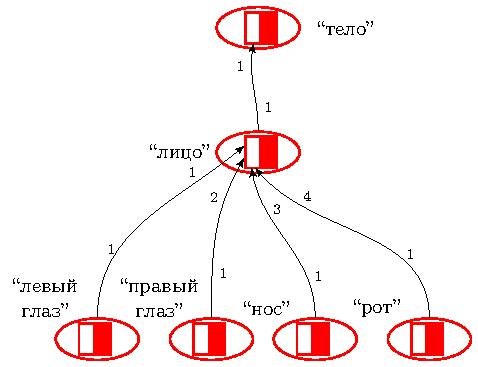
\includegraphics[page=1,width=0.6\textwidth]{examples/causnet/caus_net_colored}
		\includegraphics[width=0.4\textwidth]{misc/photos/face}
	
		\nocite{*}
		\printbibliography[keyword={signopernew}, resetnumbers=true]
	\end{frame}

	\begin{frame}
		\frametitle{Каузальная сеть на значениях: пример}
		
		\begin{figure}
			\includegraphics[page=2,width=0.7\textwidth]{examples/causnet/caus_net_colored}
		\end{figure}
		
	\end{frame}

	\begin{frame}
		\frametitle{Каузальная сеть на личностных смыслах: пример}
		
		\begin{figure}
			\includegraphics[page=3,width=0.7\textwidth]{examples/causnet/caus_net_colored}
		\end{figure}
		
	\end{frame}	

	\subsection{Семиотическая сеть}

	\begin{frame}
		\frametitle{Картина мира субъекта деятельности}
		
		\begin{columns}
			\begin{column}{0.45\textwidth}
				\begin{figure}
					\includegraphics[width=\textwidth]{signnet/signs_net}
				\end{figure}
			\end{column}
			\begin{column}{0.55\textwidth}
				\scriptsize
				\textbf{Знаком} будем называть четверку $s=\langle n,p,m,a\rangle$, где $n$ - имя знака,  $p=Z^p, m=Z^m,a=Z^a$ - кортежи каузальных матриц, которые соответственно называются образом, значением и личностным смыслом знака $s$.
				\par\medskip
				\textbf{Семиотическая сеть} - пятерка $\Omega=\langle W_p, W_m, W_a, R_n, \Theta, \Phi\rangle$, где
				\begin{itemize}
					\item $W_p, W_m, W_a$ - соответственно каузальные сети на множестве образов, значений и личностных смыслах,
					\item $R_n$ - семейство отношений на множестве знаков, сгенерированных на основе трех каузальных сетей, т.е. $R_n=\{R_p, R_m, R_a\}$,
					\item $\Theta$ - семейство операций на множестве знаков,
					\item $\Theta$ - правила распространения активности на каузальных сетях.
				\end{itemize}
			\end{column}
		\end{columns}
		\nocite{*}
		\printbibliography[keyword={symbsign}, resetnumbers=true]
	\end{frame}	
